\chapter{Simulations and Results}
For all simulations, a 1000x1000 square is used to represent the whole 2-D plane. This size is good enough in the sense that using a larger square led to longer runtimes with little to no 
effect on the results. In the mobility model we used, transition length is Rayleigh distributed. To draw a length from Rayleigh distribution, the following method is used:

\begin{enumerate}
	\item Draw a number N from Poisson distribution with density $\lambda A$ where $A$ is the area of the square.
	\item Distribute these N points uniformly on the square 
	\item Of these N points, choose the point that is closest to the point under consideration. 
\end{enumerate}

As discussed in \cite{ganti}, this leads to Rayleigh distribution of transition length and can be proved easily using null probability of a Poisson Point Process. 

\section{$E[L]$}
To test if the above mentioned method introduces any artefacts, let us see how simulated $E[L]$ fares with the formula $E[L] = \frac{1}{2\sqrt{\lambda}}$. Simulated expected length is calculated by averaging transition lengths of 100 traces in each of which the node makes 1000 transitions. 
\begin{figure}[h]
	\centering \vspace{-0.1in}
	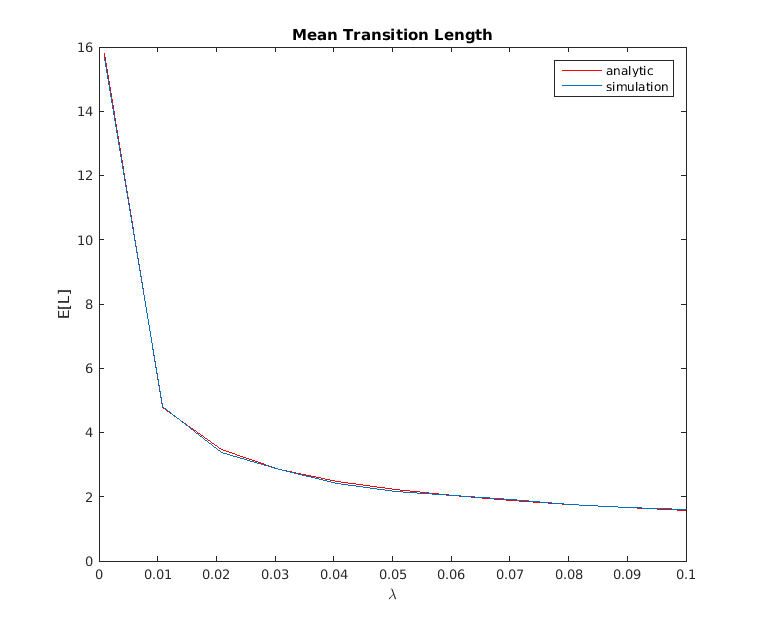
\includegraphics[width=0.75\textwidth]{images/rwpStat.png}
	\vspace{-20pt} \caption[Mean transition length vs. $\lambda$]{Mean transition length vs. $\lambda$}
	\label{fig:rwpEL}
\end{figure}
As seen in the graph \ref{fig:rwpEL}, the simulated value closely follows the analytical formula.
\section{$\rho(r,\theta)$}
In this section we look at how the probability $\rho(r,\theta)$ of moving out in one step varies in the region i.e., for different $r$ and $\theta$ and with the mobility parameter $\lambda$. 

\subsection{$\rho(r,\theta)$ vs. $\lambda$}

The plots in figure \ref{fig:vslambda} are for points inside the region and along the line joining centers of circles. At each iteration the node is placed at $(r,0)$ and a PPP($\lambda$) is generated. Probability is calculated by taking expected value of the indicator random variable which takes value 1 if the nearest point in PPP is outside the region and 0 if it is inside the region. 
\begin{figure}[ht!]
     \begin{center}
%
        \subfigure[$\lambda = 0.0005$]{%
            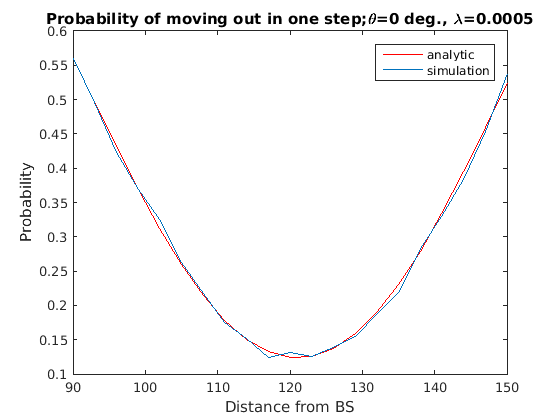
\includegraphics[width=0.6\textwidth]{images/oneOutProbl0005t0.png}
        }%
        \subfigure[$\lambda = 0.001$]{%
           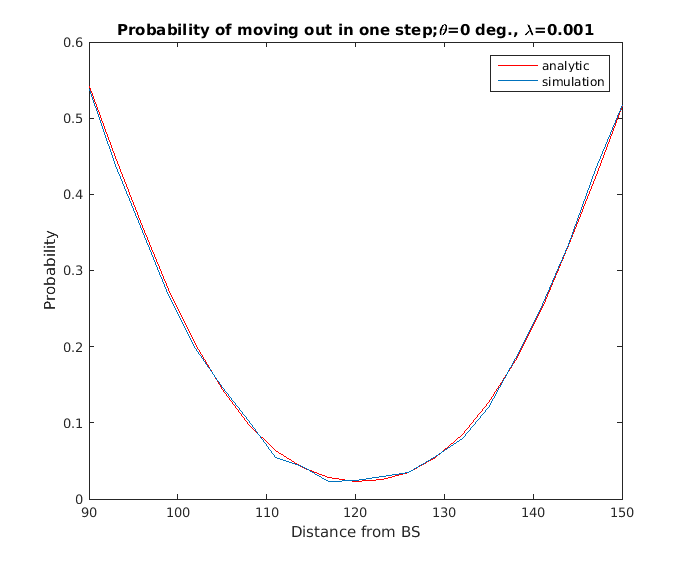
\includegraphics[width=0.55\textwidth]{images/oneOutProbl001t0.png}
        }\\ %  ------- End of the first row ----------------------%
        \subfigure[$\lambda = 0.005$]{%
            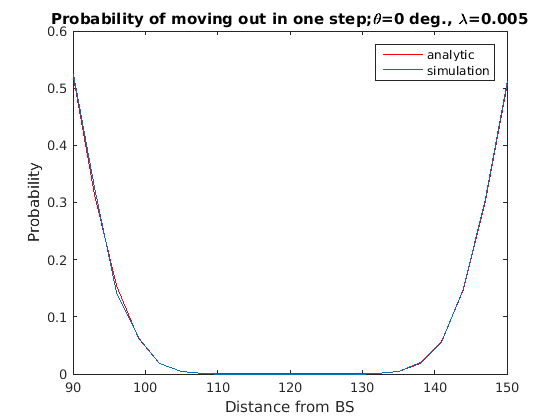
\includegraphics[width=0.6\textwidth]{images/oneOutProbl005t0.png}
        }%

%        \subfigure[Caption of Fourth Figure]{%
%            \label{fig:fourth}
%            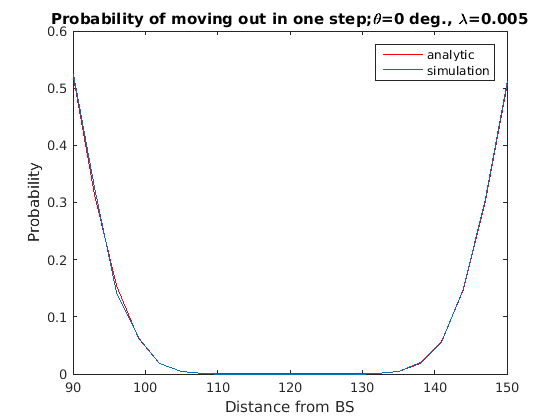
\includegraphics[width=0.4\textwidth]{images/oneOutProbl005t0.png}
        %}%
%
    \end{center}
	\caption[$\rho(r,0)$ vs. $\lambda$]{\small $\rho(r,0)$ vs. $ \lambda$}%
   \label{fig:vslambda}
\end{figure}
What we can observe in figure \ref{fig:vslambda} is that the probability for the points well within the region decreases as $\lambda$ is increased. For points near the boundary of the region, the probability doesn't change significantly. This is in line with what is expected. For points well inside the region, $E[L]$ primarily decides whether or not they leave the region and for points closer to the boundary, the probability depends on the choice of angle $\alpha$.
\subsection{$\rho(r,\theta)$ for different $\theta$}
\begin{comment}
\begin{figure}[h]
	\centering \vspace{-0.1in}
	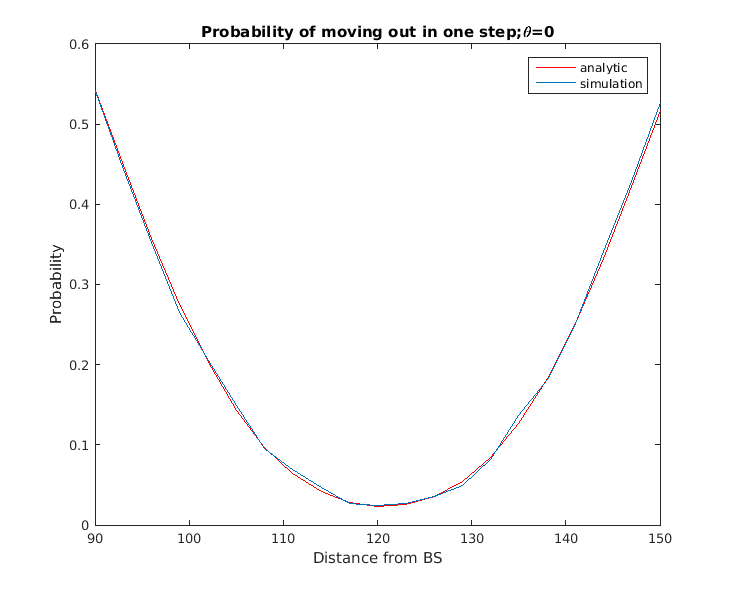
\includegraphics[width=0.75\textwidth]{images/oneOutProb0.png}
	\vspace{-20pt} \caption[Effect of the proximal Operator]{\small Effect of the Proximal Operator }
	\label{fig:oneOut0}
\end{figure}

\begin{figure}[h]
	\centering \vspace{-0.1in}
	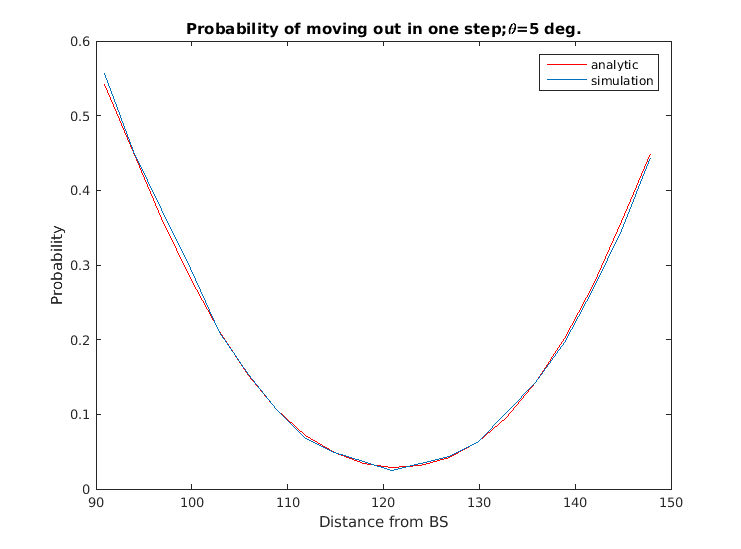
\includegraphics[width=0.75\textwidth]{images/oneOutProb5.png}
	\vspace{-20pt} \caption[Effect of the proximal Operator]{\small Effect of the Proximal Operator }
	\label{fig:oneOut5}
\end{figure}

\begin{figure}[h]
	\centering \vspace{-0.1in}
	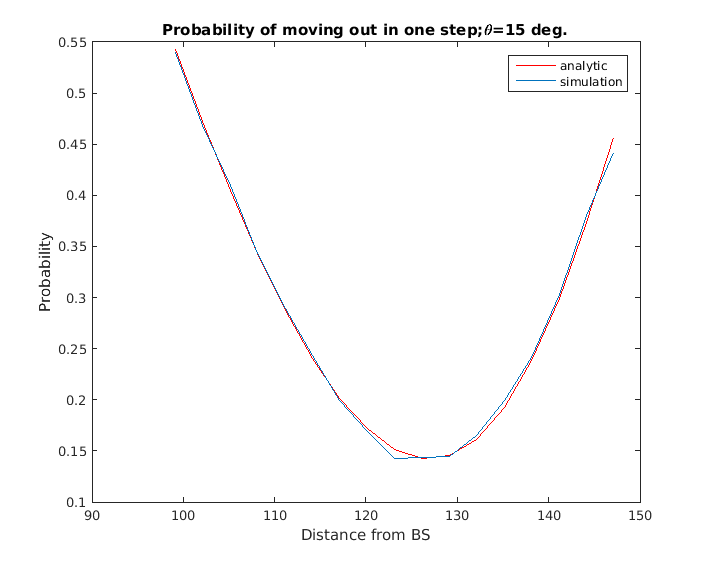
\includegraphics[width=0.75\textwidth]{images/oneOutProb15.png}
	\vspace{-20pt} \caption[Effect of the proximal Operator]{\small Effect of the Proximal Operator }
	\label{fig:oneOut15}
\end{figure}

\begin{figure}[h]
	\centering \vspace{-0.1in}
	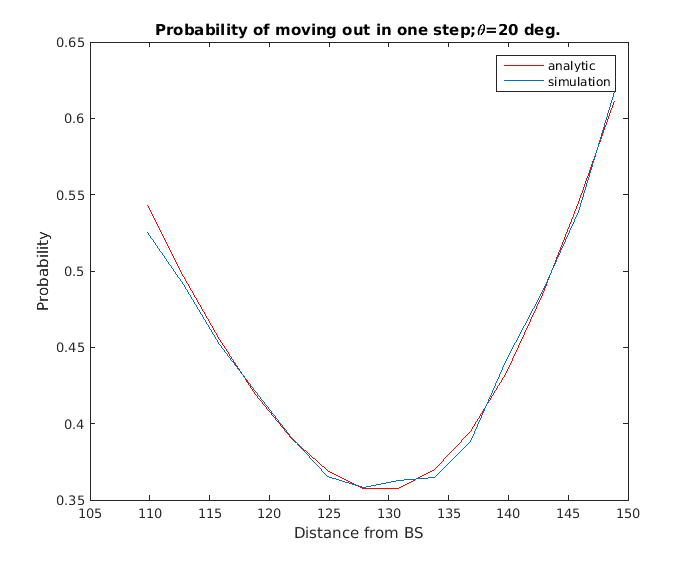
\includegraphics[width=0.75\textwidth]{images/oneOutProb20.png}
	\vspace{-20pt} \caption[Effect of the proximal Operator]{\small Effect of the Proximal Operator }
	\label{fig:oneOut20}
\end{figure}
\end{comment}

Figure \ref{fig:vangles} shows how $\rho(r,\theta)$ along the radius changes with $\theta$. We can see that it increases with $\theta$ for points inside the region and doesn't change significantly for points at the edges. We can see that the maximum can occur at both edges.

\begin{figure}[H]
     \begin{center}
%
		 \subfigure[$\theta = 0^{\circ}$]{%
            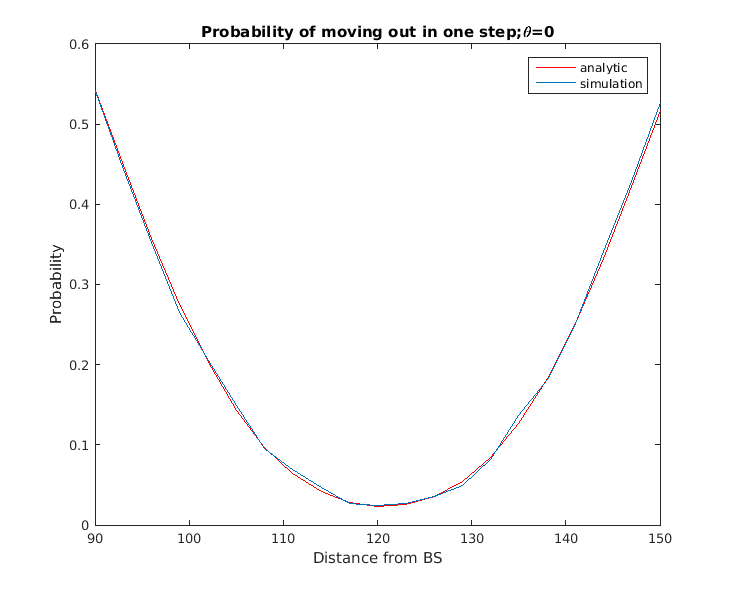
\includegraphics[height = 2.5in,width=3.5in]{images/oneOutProb0.png}
        }%
        \subfigure[$\theta = 5^{\circ}$]{%
           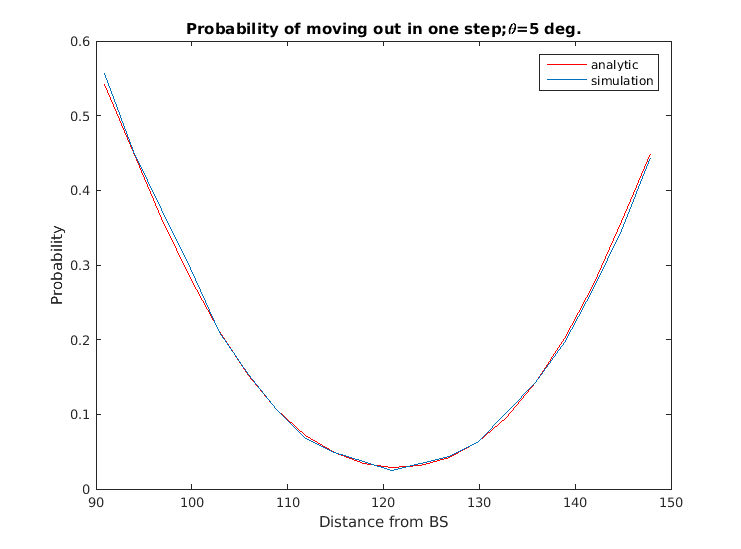
\includegraphics[height = 2.5in,width=3.5in]{images/oneOutProb5.png}
        }\\ %  ------- End of the first row ----------------------%
        \subfigure[$\theta = 15^{\circ}$]{%
            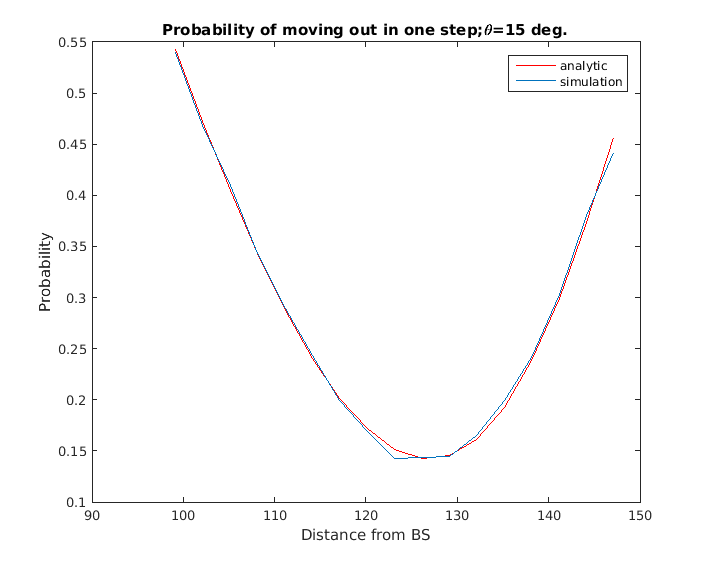
\includegraphics[height = 2.5in,width=3.5in]{images/oneOutProb15.png}
        }%

        \subfigure[$\theta = 20^{\circ}$]{%
            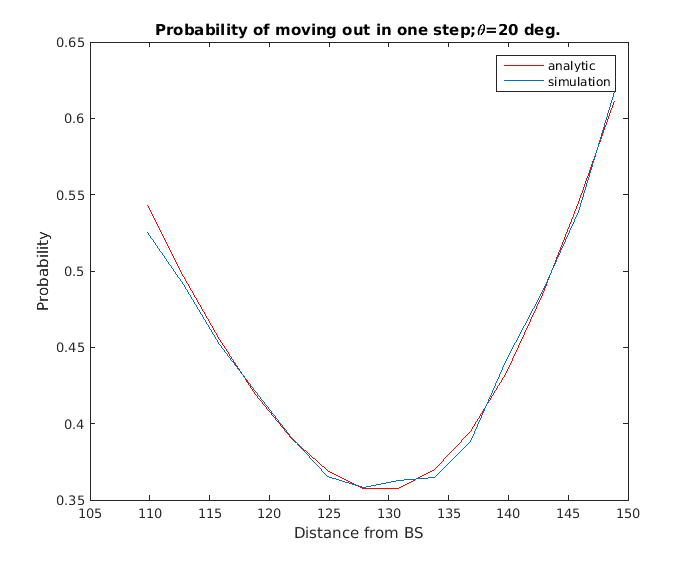
\includegraphics[height = 2.5in,width=3.5in]{images/oneOutProb20.png}
        }%
%
    \end{center}
	\caption[$\rho(r,\theta)$ at different angles]{$\rho(r,\theta)$ at different angles}%
   \label{fig:vangles}
\end{figure}
\section{E[N]}
Figure \ref{fig:EN} shows the expected number of steps in which a node leaves the region.
The plots are for points along the radius at angles $\theta = 10^{\circ}$ and $\theta = 15^{\circ}$. We can see that the analytical formula agrees better for narrower regions. As discussed in Chapter 4, this can be improved by modelling the motion of a node as an absorbing Markov Chain and discretizing the state space.

\begin{figure}[ht!]
     \begin{center}
%
		 \subfigure[$\theta = 10^{\circ}$]{%
            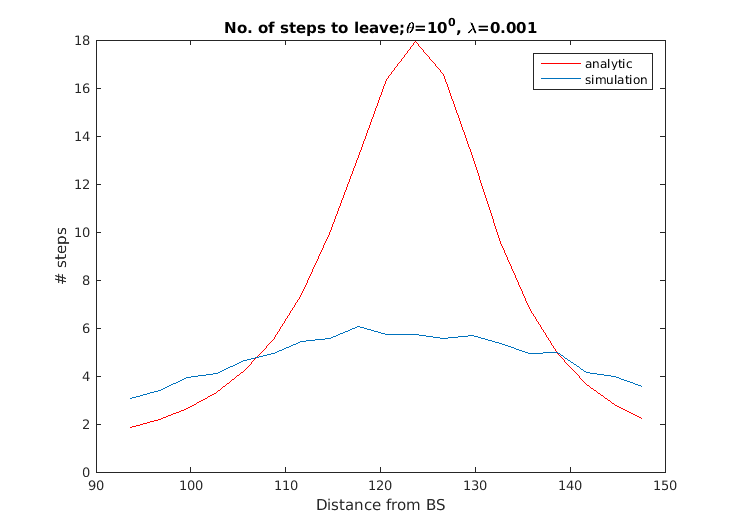
\includegraphics[height = 2.5in,width=3.5in]{images/stepst10.png}
        }%
        \subfigure[$\theta = 15^{\circ}$]{%
           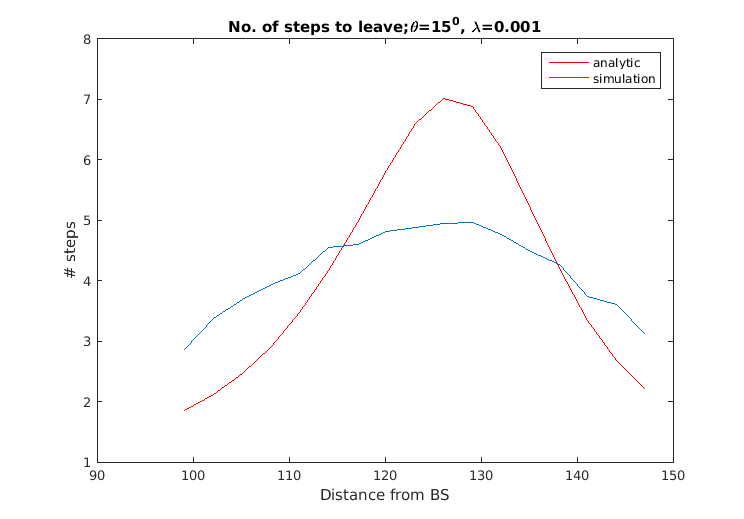
\includegraphics[height = 2.5in,width=3.5in]{images/stepst15.png}
        }\\ %  ------- End of the first row ----------------------%
%
    \end{center}
	\caption[Expected number of transitions]{Expected number of transitions}%
   \label{fig:EN}
\end{figure}





